\documentclass[14pt,a4paper]{extarticle}
\usepackage[paper=a4paper,margin=2cm]{geometry}

\usepackage{fontspec}
\setmainfont{PT Serif}
\setsansfont{PT Sans}
\setmonofont{PT Mono}

\usepackage{polyglossia}
\setdefaultlanguage{russian}
\setotherlanguage{english}
\usepackage{microtype}

\usepackage{setspace}
\singlespacing

\setlength{\parindent}{1.25cm}
\setlength{\parskip}{0pt}

\usepackage{titlesec}
\titleformat{\section}{\normalfont\Large\bfseries}{\thesection}{1em}{}
\titleformat{\subsection}{\normalfont\large\bfseries}{\thesubsection}{1em}{}

\renewcommand{\thefigure}{\thesection.\arabic{figure}}
\counterwithin{figure}{section}

\usepackage[
    colorlinks=true,      % Включить цветные ссылки
    linkcolor=black,      % Цвет ссылок
    citecolor=black,      % Цвет цитат
    urlcolor=black,       % Цвет URL
    pdfborder={0 0 0}     % Убрать рамки вокруг ссылок
]{hyperref}
\usepackage{graphicx}
\usepackage{subcaption}
\usepackage{tcolorbox}
\usepackage{tikz}
\usepackage{xcolor}
\usepackage{minted}
\usepackage{fancyvrb}
\usepackage{amsmath}
\usepackage{amsfonts}
\usepackage{amssymb}

\usepackage{enumitem}
\setlist[itemize]{label=$\bullet$}

\usepackage{tikz}
\usetikzlibrary{trees, positioning}

\setminted{
	style=friendly,
	breaklines=true,
	breaksymbol=$\hookrightarrow$,
	breakafter=,
	breakautoindent=true,
	fontsize=\small
}

\begin{document}

\begin{titlepage}
    \centering
    \begin{figure}
        \centering
        
\includegraphics[width=0.5\linewidth]{logo.png}
    \end{figure}
    {\Huge \textbf{Отчет по курсовой работе по дисциплине "Защита данных"}} \\[1cm]
    {\Large Программная реализация криптоалгоритма на основе эллиптических кривых} \\[2cm]
    \textbf{Автор:} \\[0.5cm]
    {\large Студент группы А-05-22} \\ [0.1cm]
    {\large Володченков Никита Дмитриевич} \\[1.5cm]
    \textbf{Преподаватель:} \\[0.5cm]
    {\large Хорев Павел Борисович} \\[1.5cm]

    \vfill
    \textbf{Дата:} \\[0.5cm]
    {\large \today} \\[3cm]
\end{titlepage}

\tableofcontents
\newpage

\section{Задание}

Требуется на основе криптографического алгоритма на эллиптических кривых разработать приложение со следующим функционалом:

\begin{enumerate}
    \item возможность шифровать/расшифровывать короткие сообщения на случайных (или извлекаемых из выбираемых файлов) асимметрических ключах выбираемой пользователем длины;
    \item возможность сохранения случайной пары ключей в двух файлах с задаваемыми пользователем именами (закрытый ключ должен при этом шифроваться на ключе, выводимом из специальной парольной фразы);
    \item возможность определять при расшифровании закрытого ключа факт ввода неверной парольной фразы (например, путем добавления к ключу перед его шифрованием сигнатуры – специальной строки символов – с проверкой ее наличия в расшифрованном ключе и удалением из него в случае успешной проверки).
\end{enumerate}

\section{Теория}

\subsection{Эллиптическая кривая в форме Вейерштрасса над конечным полем}

\textbf{Эллиптическая кривая} $\mathbf E$ (в форме Вейерштрасса) - это множество точек на плоскости, удовлетворяющих уравнению
%
\[
y^2 = x^3 + ax + b
\]

Изначально положим, что $a, b$ и координаты точки $x$ принадлежат полю $\mathbb R$. Также, чтобы исключить особые эллиптические кривые, требуем, чтобы $\Delta=-16(4a^3+27b^2) \neq 0$.

Интересным фактом является то, что проведя через 2 отличные прямую, получим при пересечении либо третью точку, отличную от предыдущих двух, либо эта прямая будет касательной к этой кривой. По следующему правилу может быть определена группа:

\begin{enumerate}
    \item Элементами группы являются точки на эллиптической кривой $E$: $\{(x, y) \in E : x, y \in \mathbb F\}$, где $\mathbb F$ - некоторое поле, пока рассматриваем $\mathbb R$
    \item К этим точкам добавим некоторую бесконечно удаленную точку, которую обозначим за $0$ и будем считать её нейтральным элементом группы
    \item Если $P, Q, R$ - точки на эллиптической кривой, лежащие на одной прямой, то $P+Q+R=0$
    \item Если эта прямая касается эллиптической кривой, то точку касания считаем дважды (то есть если прямая касается эллиптической кривой в точке $P$ а также проходит через точку $Q$, то $P+P+Q=0$)
    \item Если $R=(x, y)$, то $-R=(x, -y)$
\end{enumerate}

Доказывается, что такие правила действительно дают нам группу. Тогда, например координаты точки $R=P+Q$ ($x_P\neq x_Q$) могут быть вычислены по следующим формулам
%
\begin{align*}
    s &= \frac{y_P - y_Q}{x_P - x_Q} \\
    x_R &= s^2 - x_P - x_Q \\
    y_R &= -y_P + s(x_P - x_R)
\end{align*}

Если $x_P=x_Q$, то либо $y_P=-y_Q$, значит $P+Q=0$, либо $P=Q$, тоесть $R=2P$, тогда через точку $P$ требуется провести касательную, и получим такие формулы
%
\begin{align*}
    s &= \frac{3x_P^2+a}{2y_P} \\
    x_R &= s^2 - 2x_P \\
    y_R &= -y_P + s(x_P - x_R)
\end{align*}

Тут видна проблема, когда $y_p=0$. Геометрически это означает, что касательная к точке вертикальна, а значит получаем бесконечно удаленную точку, которую в группе условились называть точкой $0$. Таким образом, можем выделить 2 способа получения точки $0$ в эллиптической группе:

\begin{itemize}
    \item Если $x_P=x_Q$ и $y_P=-y_Q$, то $P+Q=0$
    \item Если $x_P=x_Q$ и $y_P=y_Q=0$, то $P+Q=0$
\end{itemize}

Теперь можем перейти к конечному полю $\mathbb F_p$ (полю целых чисел по простому вычету $p$). Если сохраним те же формулы, что определены геометрически, то оказывается, что точки до сих пор образуют группу. Далее за $E(\mathbb F_p)$ будем обозначать построенную ранее группу точек на эллиптической кривой в поле $\mathbb F_p$.

\subsection{Проблема дискретного логарифма на эллиптических кривых (ECDLP)}

Основанием для надежности криптографического алгоритма на эллиптических кривых является проблема дискретного логарифма на эллиптических кривых. Формулировка проблемы звучит так:

\begin{tcolorbox}[title=Elliptic Curve Discrete Logarithm Problem]
    Рассматриваются точки из $E(\mathbb F_p)$. Известно, что $Q=kP$ (за $kP$ обозначается $k$-кратное повторение сложения точки $P$). Требуется, зная $Q$ и $P$, определить $k$.
\end{tcolorbox}

Рассмотрим подгруппу $\langle P \rangle = \{mP: m=1,2,3,\dots\}$. Обозначим её порядок за $n$.

в этот раздел еще добавлю потом про то что требуется очень много времени для решения этой проблемы а также случаи когда эта проблема решается быстро и какой класс эллиптических кривых не используется из-за этого на практике

\subsection{Зашифрованная передача точки эллиптической кривой}

Для этого буду использовать схему с публичным ключом Эль-Гамаля (ElGamal Public Key Encryption). Рассмотрим пользователя $A$, который хочет отправить точку $M$ пользователю $B$ так, чтобы по незащищенному каналу её определить было невозможно. Перед началом передачи пользователи договариваются об эллиптической кривой $E(\mathbb F_p)$ и точки этой эллиптической кривой $G$.

Пользователь $B$ будет располагать секретным ключом $s$, по которому формирует открытый ключ $P=sG$, который может предоставить любому пользователю, который хочет передать ему сообщение. Например, пользователь $A$ должен сделать следующее:

\begin{enumerate}
    \item Получить открытый ключ $P$
    \item По случайно выбранному значению $k$ вычислить точку $M_1=kG$
    \item Вычислить точку $M_2=M+kP$
    \item Отправить по открытому каналу пользователю $B$ точки $M_1$ и $M_2$
\end{enumerate}

По этим точкам пользователь $B$ может вычислить точку $M$ следующим образом:
%
\[
M_2-sM_1 = (M+kP) - s(kG) = M + k(sG) - skG = M
\]

При этом по открытому каналу передавались только следующие точки $P, M_1, M_2$, для расшифровки точки $M$ злоумышленнику (которому известны ранее выбранные $E(\mathbb F_p)$ и $G$) требуется выудить отсюда закрытый ключ $s$, который можно получить только путем решения задачи дискоретного логарифма на эллиптической кривой, благодаря чему можно судить о надежности этого метода передачи.

\subsection{Кодирование сообщения в точку эллиптической кривой}

Проблемой передачи точки из предыдущего раздела является то, что нам обычно требуется передавать не какую-то абстрактную точку эллиптической кривой, а сообщение. Передачу сообщения предыдущим методом можно организовать, если мы будем уметь кодировать произвольное сообщение в точку на эллиптической кривой и декодировать обратно. Для этого существует несколько методов, ниже приведен один из них.

\begin{tcolorbox}[title=Koblitz's Method]
    Дана эллиптическая кривая $y^2=x^3+ax+b$ над полем $\mathbb F_p$. Также дано сообщение $m$ которое требуется сопоставить точке на эллиптической кривой (требуется чтобы $0 \leq m < p/100$).

    В цикле $j=0,1,2,\dots,99$ вычисляем:
    \begin{itemize}
        \item $x_j=100m+j$
        \item $s_j = x_j^3+ax_j+b$
        \item $s_j^{(p-1)/2}\equiv 1 \pmod p \implies s_j$ - квадратный вычет по модулю $p$, следовательно процедуру можно завершить 
    \end{itemize}

    Теперь требуется вычислить $y_j$:

    \begin{itemize}
        \item Если $p \equiv 3 \pmod p$, то $y_j \equiv s_j^{(p+1)/4} \pmod p$
        \item Если $p \equiv 1 \pmod p$, то процедура намного сложнее, поэтому запретим выбирать такие простые числа
    \end{itemize}
\end{tcolorbox}

\section{Разработка приложения}

\subsection{Проект пользовательского интерфейса приложения}
 
\begin{figure}[!htbp]
    \centering
    \begin{subfigure}{0.9\textwidth}
        \centering
        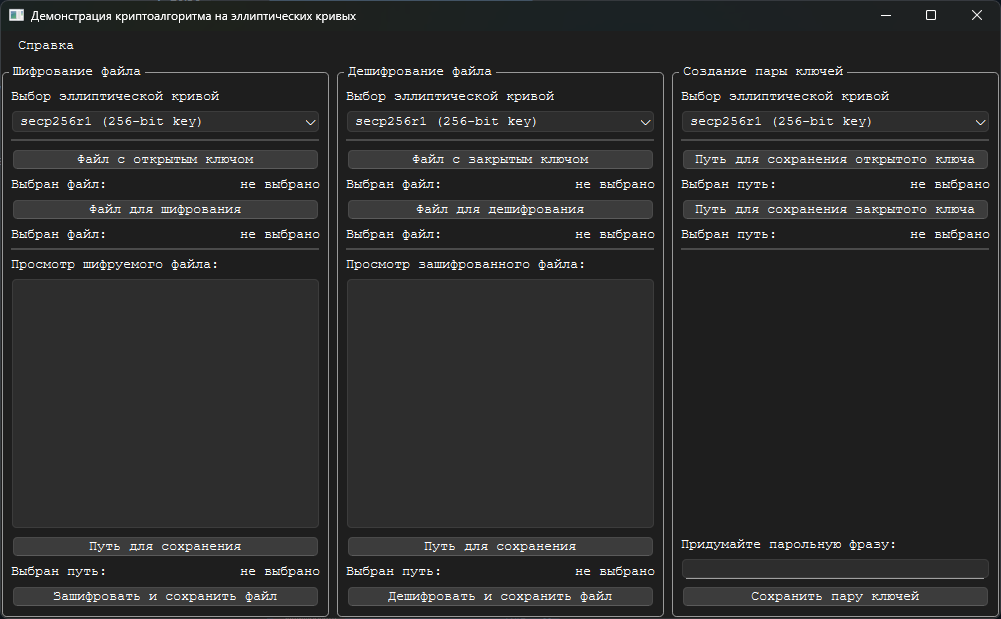
\includegraphics[width=\textwidth]{src/main_win.png}
        \caption{Общий вид главного окна при запуске программы (ничего не выбрано)}
        \label{fig:main_window_without_list}
    \end{subfigure}
    \hfill
    \begin{subfigure}{0.9\textwidth}
        \centering
        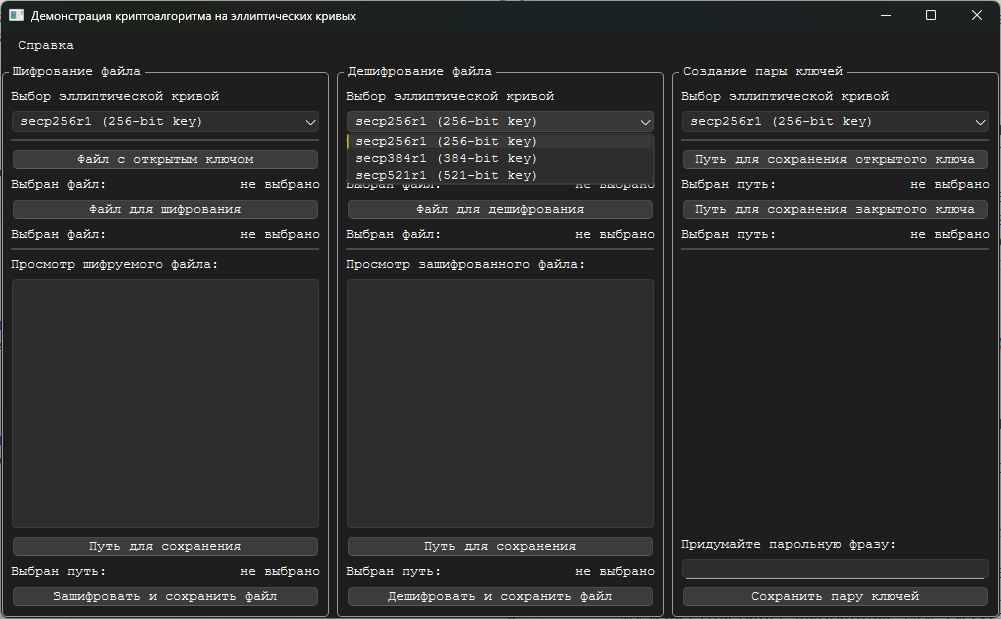
\includegraphics[width=\textwidth]{src/main_win_list.png}
        \caption{Выпадающий список по выбору длины ключа и эллиптической кривой}
        \label{fig:main_window_with_list}
    \end{subfigure}
    \caption{Главное окно}
\end{figure}

\begin{figure}[!htbp]
    \centering
    \begin{subfigure}{0.45\textwidth}
        \centering
        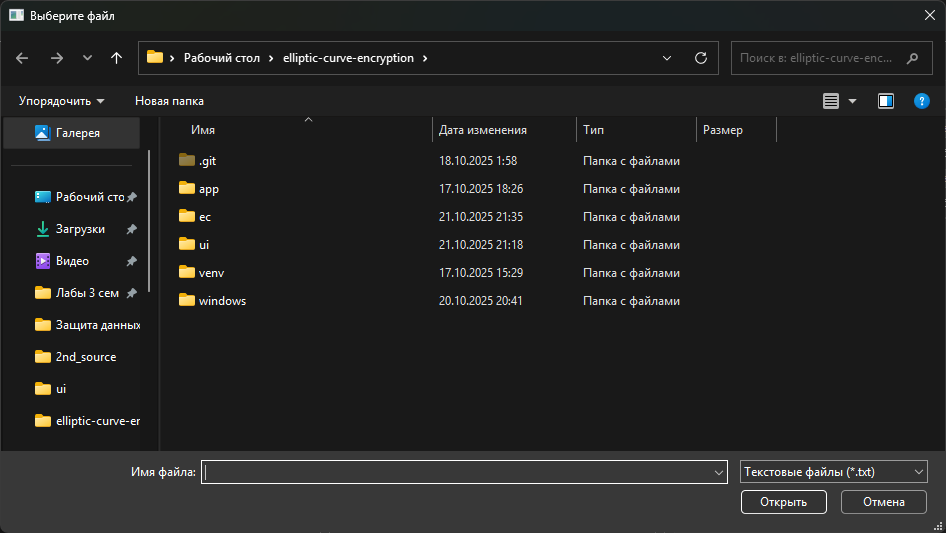
\includegraphics[width=\textwidth]{src/choose_file_win.png}
        \caption{Выбор существующего файла}
        \label{fig:choose_file_window}
    \end{subfigure}
    \hfill
    \begin{subfigure}{0.45\textwidth}
        \centering
        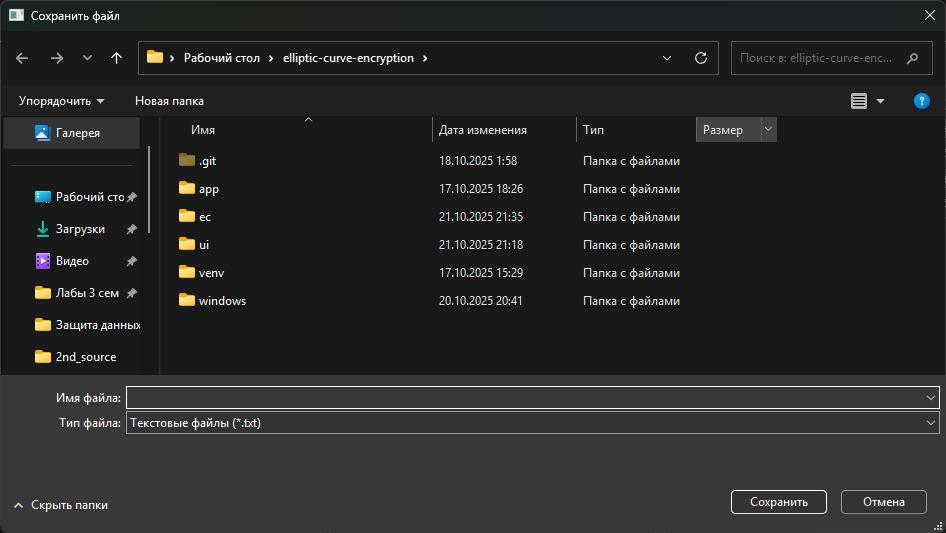
\includegraphics[width=\textwidth]{src/save_file_win.png}
        \caption{Выбор пути сохранения файла}
        \label{fig:save_file_window}
    \end{subfigure}
    \caption{Окна по выбору путей файлов}
\end{figure}

\begin{figure}[!htbp]
    \centering
    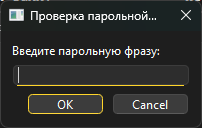
\includegraphics[scale=1]{src/passphrase_win.png}
    \caption{Окно ввода парольной фразы}
    \label{fig:passphrase_window}
\end{figure}

Главное приложение окна представлено на рисунке \ref{fig:main_window_without_list}. Оно поделено на 3 секции:

\begin{itemize}
    \item \textbf{Шифрование файла.} В этом разделе есть возможность выбрать эллиптическую кривую, которая будет использоваться при шифровании файла, файл, содержащий в себе открытый ключ и файл, который надо зашифровать. Когда выбран файл для шифрования будет показываться его содержимое. Также требуется выбрать путь по которому будет сохранена зашифрованная версия файла.
    \item \textbf{Дешифрование файла.} Аналогично предыдущему разделу, только теперь надо выбрать файл с зашифрованным закрытым ключом и файл который требуется расшифровать. Содержимое зашифрованного файла также будет отображаться на экране. После того как будет нажата кнопка "Дешифровать и сохранить файл" откроется окно, изображенное на рисунке \ref{fig:passphrase_window}, которое ждет ввода парольной фразы, требующейся для расшифрования закрытого ключа.
    \item \textbf{Создание пары ключей.} Последний раздел отвечает за случайную генерацию пары ключей для определенной эллиптической кривой. А также здесь выбирается парольная фраза, которая будет использоваться для шифрования закрытого ключа.
\end{itemize}

На рисунке \ref{fig:main_window_with_list} также изображен выпадающий список эллиптических кривых. Пока что там представлено всего 3 эллиптических кривых, которых в итоговом проекте скорее всего будет больше. Этот выбор влияет в том числе на длину открытого и закрытого ключей.

На рисунках \ref{fig:choose_file_window} и \ref{fig:save_file_window} изображены окна, которые будут открываться при нажатии на кнопки "Файл ..." (например, "Файл с закрытым ключом") и "Путь ..." (например, "Путь для сохранения") соответственно для выбора существующего файла для открытия или пути сохранения нового файла.

\subsection{Используемые средства разработки}

Для разработки выбрал язык \texttt{Python}, никаких дополнительных криптографических библиотек использоваться не будет. Скорее всего будут функции библиотеки \texttt{numpy} или подобных для арифметики, \texttt{matplotlib} для тестирования.

Для разработки пользовательского интерфейса - \texttt{PyQt6}.

\section{Тестирование}

\newpage
\nocite{washington2008elliptic}
\nocite{neuromancer_std_curves}
\bibliographystyle{ugost2008}
\bibliography{refs}   % имя .bib файла (без расширения)
\addcontentsline{toc}{section}{Список литературы}

\end{document}
